\begin{figure}[!htbp]\centering
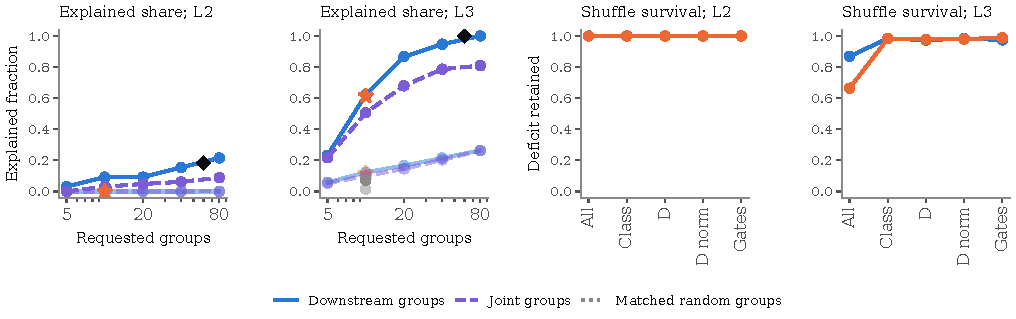
\includegraphics[width=6.098in]{cluster_pairings.pdf}
\caption{Grouping and pairing tests in the width-128 ReLU MLP, seed 0. Left pair: deficit explained as the requested group count changes; light and dark curves denote high accuracy and epoch 500. Stars mark class groups and diamonds suffix-gate patterns, at their actual group count. Right pair: deficit remaining after global shuffles (All) or shuffles within classes, downstream groups (D), normalized downstream groups (D norm), or suffix-gate groups; blue is high accuracy and orange epoch 500. The L2 deficit survives almost entirely; L3 is more sensitive to global shuffling than to shuffling within groups.}\label{fig:mechanism}
\end{figure}
\FloatBarrier
